%%%%%%%%%%%%%%%%%%%%%%%%%%%%%%%%%%%%%%%%%
% TU Muenchen 17 Sommer Semester 
% Biologically-inspired Learning of Humanoide Roboters
% 
% Advantages and Drawbacks of MLP and CMAC
%%%%%%%%%%%%%%%%%%%%%%%%%%%%%%%%%%%%%%%%%

%----------------------------------------------------------------------------------------
%	PACKAGES AND OTHER DOCUMENT CONFIGURATIONS
%----------------------------------------------------------------------------------------

\documentclass[
11pt, % Main document font size
a4paper, % Paper type, use 'letterpaper' for US Letter paper
oneside, % One page layout (no page indentation)
%twoside, % Two page layout (page indentation for binding and different headers)
headinclude%footinclude, % Extra spacing for the header and footer
BCOR3mm, % Binding correction
]{scrartcl}

%%%%%%%%%%%%%%%%%%%%%%%%%%%%%%%%%%%%%%%%%
% Arsclassica Article
% Structure Specification File
%
% This file has been downloaded from:
% http://www.LaTeXTemplates.com
%
% Original author:
% Lorenzo Pantieri (http://www.lorenzopantieri.net) with extensive modifications by:
% Vel (vel@latextemplates.com)
%
% License:
% CC BY-NC-SA 3.0 (http://creativecommons.org/licenses/by-nc-sa/3.0/)
%
%%%%%%%%%%%%%%%%%%%%%%%%%%%%%%%%%%%%%%%%%

%----------------------------------------------------------------------------------------
%	REQUIRED PACKAGES
%----------------------------------------------------------------------------------------

\usepackage[
nochapters, % Turn off chapters since this is an article        
beramono, % Use the Bera Mono font for monospaced text (\texttt)
eulermath,% Use the Euler font for mathematics
pdfspacing, % Makes use of pdftex’ letter spacing capabilities via the microtype package
dottedtoc % Dotted lines leading to the page numbers in the table of contents
]{classicthesis} % The layout is based on the Classic Thesis style

\usepackage{arsclassica} % Modifies the Classic Thesis package

\usepackage[T1]{fontenc} % Use 8-bit encoding that has 256 glyphs

\usepackage[utf8]{inputenc} % Required for including letters with accents

\usepackage{graphicx} % Required for including images
\graphicspath{{Figures/}} % Set the default folder for images

\usepackage{enumitem} % Required for manipulating the whitespace between and within lists

\usepackage{lipsum} % Used for inserting dummy 'Lorem ipsum' text into the template

\usepackage{subfig} % Required for creating figures with multiple parts (subfigures)

\usepackage{amsmath,amssymb,amsthm} % For including math equations, theorems, symbols, etc

\usepackage{varioref} % More descriptive referencing

%----------------------------------------------------------------------------------------
%	THEOREM STYLES
%---------------------------------------------------------------------------------------

\theoremstyle{definition} % Define theorem styles here based on the definition style (used for definitions and examples)
\newtheorem{definition}{Definition}

\theoremstyle{plain} % Define theorem styles here based on the plain style (used for theorems, lemmas, propositions)
\newtheorem{theorem}{Theorem}

\theoremstyle{remark} % Define theorem styles here based on the remark style (used for remarks and notes)

%----------------------------------------------------------------------------------------
%	HYPERLINKS
%---------------------------------------------------------------------------------------

\hypersetup{
%draft, % Uncomment to remove all links (useful for printing in black and white)
colorlinks=true, breaklinks=true, bookmarks=true,bookmarksnumbered,
urlcolor=webbrown, linkcolor=RoyalBlue, citecolor=webgreen, % Link colors
pdftitle={}, % PDF title
pdfauthor={\textcopyright}, % PDF Author
pdfsubject={}, % PDF Subject
pdfkeywords={}, % PDF Keywords
pdfcreator={pdfLaTeX}, % PDF Creator
pdfproducer={LaTeX with hyperref and ClassicThesis} % PDF producer
} % Include the structure.tex file which specified the document structure and layout

\hyphenation{Fortran hy-phen-ation} % Specify custom hyphenation points in words with dashes where you would like hyphenation to occur, or alternatively, don't put any dashes in a word to stop hyphenation altogether

%----------------------------------------------------------------------------------------
%	TITLE AND AUTHOR(S)
%----------------------------------------------------------------------------------------

\title{\normalfont\spacedallcaps{comparison between MLP $\&$ CMAC}} % The article title
\author{\spacedlowsmallcaps{Group A }} % The article author(s) - author affiliations need to be specified in the AUTHOR AFFILIATIONS block
\date{Tianming Qiu,\quad Qiuhai Guo} % An optional date to appear under the author(s)

%----------------------------------------------------------------------------------------

\begin{document}

%----------------------------------------------------------------------------------------
%	HEADERS
%----------------------------------------------------------------------------------------

\renewcommand{\sectionmark}[1]{\markright{\spacedlowsmallcaps{#1}}} % The header for all pages (oneside) or for even pages (twoside)
%\renewcommand{\subsectionmark}[1]{\markright{\thesubsection~#1}} % Uncomment when using the twoside option - this modifies the header on odd pages
\lehead{\mbox{\llap{\small\thepage\kern1em\color{halfgray} \vline}\color{halfgray}\hspace{0.5em}\rightmark\hfil}} % The header style

%\pagestyle{scrheadings} % Enable the headers specified in this block

\maketitle % Print the title/author/date block

%----------------------------------------------------------------------------------------
%	MLP
%----------------------------------------------------------------------------------------

\section{MLP}

%A statement\footnote{Example of a footnote} requiring citation \cite{Figueredo:2009dg}.
\paragraph{Advantages}
\begin{itemize}[noitemsep]
\item \textbf{Better prediction}
A regression equation will be obtained so that robot can perform much better during the prediction in term of the continuity of movements.
\end{itemize} 
\paragraph{Disadvantages}
\begin{itemize}[noitemsep]
\item \textbf{Complex algorithm}
MLP algorithm includes both feedforward and backpropagation processes, what results in longer code than CMAC. 
Since there are lots of subscripts, it tends to be more easily to make mistakes during programing.

\item \textbf{Converge slowly}
It takes more than 6 million iterations and 3 minutes to make the MSE converge into its threshold.
\end{itemize} 
 
%----------------------------------------------------------------------------------------
%	CMAC
%----------------------------------------------------------------------------------------

\section{CMAC}
\paragraph{Advantages}
\begin{itemize}[noitemsep]
\item \textbf{Simple model}
The code is much shorter and structure is simpler.

\item \textbf{Converge fast}
Compared with MLP, it takes only hundreds iterations to converge into a even smaller threshold.
\end{itemize} 

\paragraph{Disadvantages}
\begin{itemize}[noitemsep]
\item \textbf{Huge demand on training data}
Because we adopt a layer 2 with resolution as 50, fast 2500 parameters need to be calculated, 
unless we cannot cover enough states. For example, in figure~\vref{fig:gallery1}, 
it shows the coverage area of receptive fields on the layer 2 with 250 samples. 
The grid board describes the 50 x 50 layer 2 and each square means a neuron.
The darker the area is, the more times it has been selected to be activated. 
When we collected those 250 samples, 
we just ‘scanned’ the red object subtly in order to cover possible more neurons on the layer 2, 
which the trajectory could even be observed clearly in the figure~\vref{fig:gallery1}. 
Unfortunately, it still remains lots of blank areas.

 
Next, we try to collect more data up to more than 850 samples. This time layer 2 seems to be totally black, 
which is shown in figure~\vref{fig:gallery1}. 
However, from neuron level, the situation is still not be optimistic. 
Apart from the area near boundary, many ‘empty neurons’ can be observed obviously from figure~\vref{fig:gallery3}. 
That means, during the prediction process, if a new data from layer 1 was going to activate a set of neurons that have never been trained before, 
the robot arm was not able to give a correct response and even ran into a not safe position.
\begin{figure}[tb]
\centering 
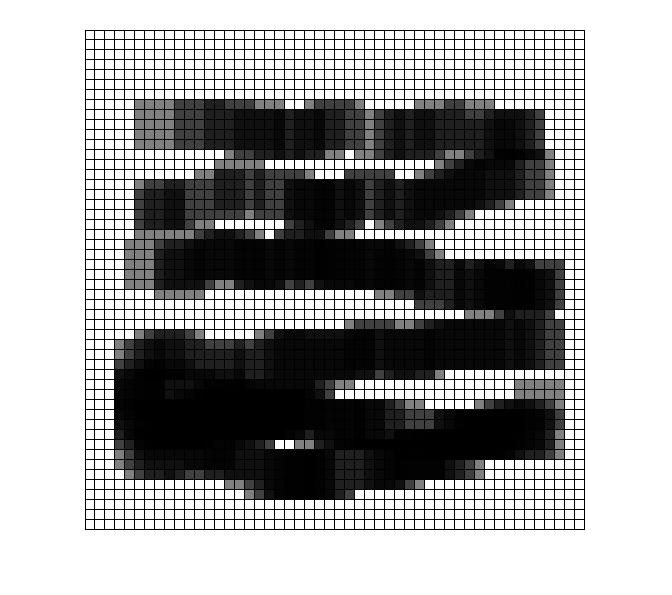
\includegraphics[width=0.45\columnwidth]{receptivefield250}
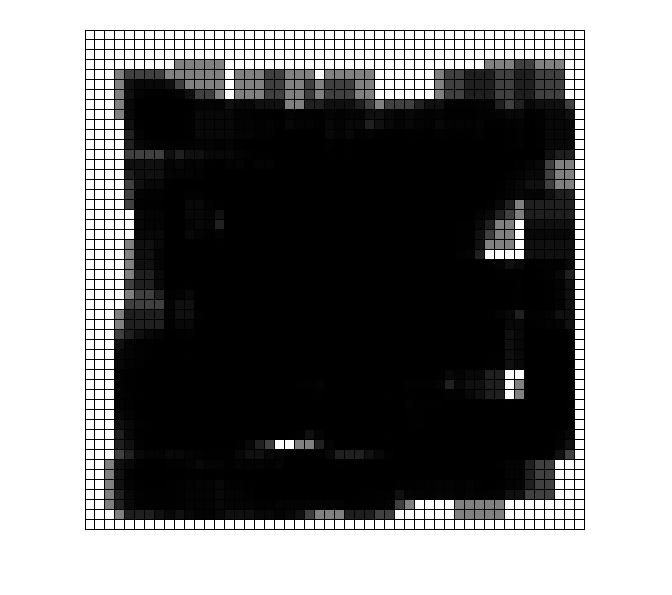
\includegraphics[width=0.45\columnwidth]{receptivefield} 
\caption[An example of a floating figure]{Coverage area (left: 250 samples right: 850 samples)} % The text in the square bracket is the caption for the list of figures while the text in the curly brackets is the figure caption
\label{fig:gallery1} 
\end{figure}

\begin{figure}[tb]
\centering 
 
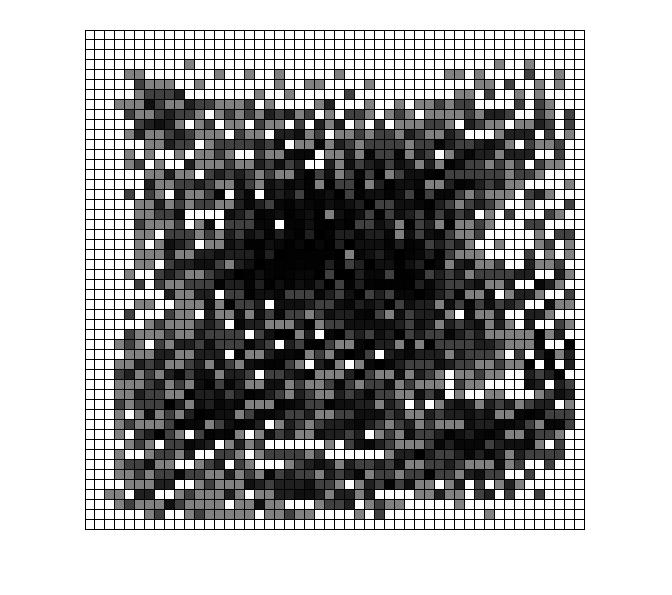
\includegraphics[width=0.8\columnwidth]{trained_neuron}
\caption[An example of a floating figure]{Activated neurons (850 samples)} % The text in the square bracket is the caption for the list of figures while the text in the curly brackets is the figure caption
\label{fig:gallery3} 
\end{figure}
\item \textbf{Lack of continuity \& weak robustness}
Since the neurons on layer 2 are discrete and the resolution has a limit of only 50, 
robot cannot trace a red object continuously, more stiff than how it perform by MLP. 
And sometimes go into wrong positions because of lack of training data in some specific areas.


\end{itemize}




\end{document}